\chapter{Grundlagen}

\section{Maschinelles Lernen (Machine Learning)}

    Wenn man maschinelles Lernen oder Künstliche Intelligenz hört, denkt die Mehrzahl an Roboter mit eigenem Bewusstsein und Denken wie in vielen Science-Fiction-Filmen dargestellt.
    Jedoch ist maschinelles Lernen mittlerweile keine Zukunftstechnologie mehr.
    Bereits in den 60er Jahren gab es erste Versuche der Wissenschaft Künstliche Intelligenz zu erschaffen.
    Doch was ist maschinelles Lernen wirklich? Und was bedeutet es für einen Computer zu lernen?
    \newline

    \noindent
    Dieses Kapitel beschäftigt sich mit diesen Fragen und gibt einen kurzen Überblick über heutige Verfahren von maschinellem Lernen.

    \subsection{Künstliche Intelligenz}
    Bevor maschinelles Lernen erklärt werden kann sollte Künstliche Intelligenz im Allgemeinen geklärt werden.


    \subsection{Einführung}
    Nimmt man den Begriff maschinelles Lernen wörtlich beschreibt er das Lernen einer Maschine, also die Fähigkeit einer Maschine intelligenter zu werden.
    Von maschinellem Lernen spricht man, falls eine Maschine auf Basis von Erfahrung und Fakten "`ohne speziell programmiert worden zu sein"'\cite[20]{HandsOnML}, neues Wissen oder neue Zusammenhänge generieren kann.
    Wenn eine Maschine, nachdem sie etwas gelernt hat, bei der Ausführung einer Aktivität besser geworden ist, hat diese etwas neues gelernt\cite[20]{HandsOnML}.
    Das reine auswendig lernen von Fakten, wie beispielsweise das Abspeichern einer Wikipedia-Seite auf die lokale Festplatte eines Computers, ist kein Wissenserwerb.
    \newline

    \noindent
    Ein Beispiel für maschinelles Lernen ist der Spamfilter bei Emails.
    Hier lernt ein Computer auf Basis von bisherigen Spammails neue Emails als Spam zu erkennen.
    \newline

    Der Einsatz von maschinellem Lernen hat meist Vorteile gegenüber herkömmlichen statistischen Methoden wenn große Datenmengen ausgewertet werden müssen oder kein bekanntes Modell zur Problemlösung bekannt ist.
    Durch maschinelles Lernen können Zusammenhänge erkannt werden, die durch andere statistische oder algorithmische Verfahren nicht erkannt oder abgebildet werden können.

    \subsection{Lernprozess} \label{Lernprozess}
    Grundlegend besteht maschinelles Lernen aus einer Trainingsphase und einer Test- beziehungsweise Validierungsphase.
    Hierzu werden zunächst alle vorhandenen Daten in Trainings- sowie Testdaten, meist im Verhältnis 80:20, eingeteilt.
    In der Trainingsphase wird auf Basis der Trainingsdaten, wie zum Beispiel bisherige Emails eines Benutzers, ein Modell erstellt, welches dann in der Validierungsphase auf seine Genauigkeit und Validierungsgenauigkeit überprüft wird.
    Genauigkeit bedeutet, dass in der Validierungsphase alle Daten, welche auch im Trainingsprozess verwendet wurden, von dem neuen Modell klassifiziert werden.\\


    Dieses Ergebnis wird mit der bekannten Klassifizierung der Daten abgeglichen und eine Übereinstimmungswahrscheinlichkeit errechnet, welche als Genauigkeit des Modells gilt.
    Um die Validierungsgenauigkeit zu berechnen wird derselbe Prozess auch mit den Testdaten durchgeführt.
    Die Validierungsgenauigkeit ist wichtig um herauszufinden ob das entstandene Netz die Trainingsdaten nur auswendig gelernt hat oder wirklich neues Wissen generiert hat.
    Dies ist der Fall, sobald während des Trainings die Validierungsgenauigkeit immer weiter sinkt, dann spricht man von "`overfitting"' des Netzes.
    \newline

    \noindent
    Aufgrund der Ergebnisse der Validierungsphase sowie der sonstigen Wissensbasis kann eine neue Trainingsphase durchgeführt werden(vgl. \ref{fig:MLTrainigsprozess}).
    Dieser Prozess wird Epoche genannt und kann beliebig oft wiederholt werden und das Modell weiter verbessert werden.
    Das entstandene Modell stellt das neu generierte Wissen dar.

    % Abbildung zu testphasen hinzufügen
    \begin{figure}[H]
        \centering
        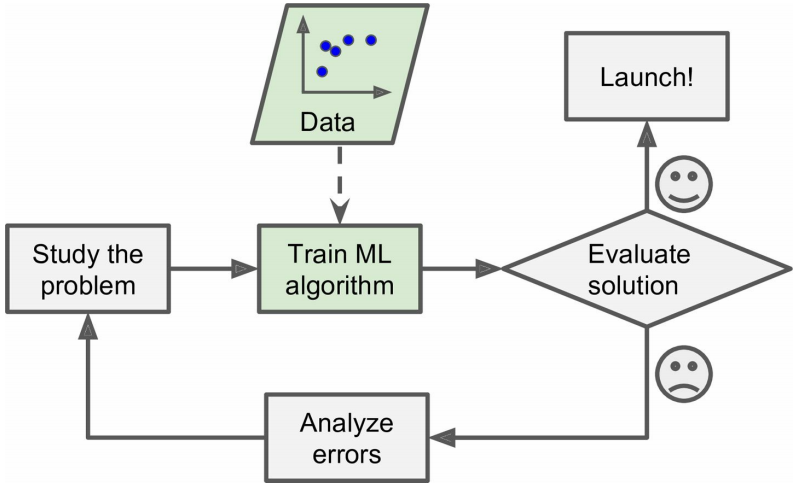
\includegraphics[width=0.8\textwidth]{MLTrainigsphasen}
        \caption{Trainingsprozess (\cite[Figure 1-2]{HandsOnML})}
        \label{fig:MLTrainigsprozess}
    \end{figure}


    \section{Neuronale Netze}
    \cite[Vgl. im Folgenden]{EinfuehrunginNN,WissensbasierteSysteme}\\
    Neuronale Netze sind eine Form von maschinellem Lernen und die heute am meisten eingesetzte Technik für Bilderkennung, Spracherkennung oder Zeitreihenanalyse.
    
    \subsection*{Aufbau}
    Ein künstliches neuronales Netz ist an das menschliche Gehirn angelehnt und soll dessen neuronales Netz sowie dessen Verhalten abbilden. 
    Dementsprechend besteht ein solches Netz aus mehreren Neuronen und Schichten von Neuronen, welche über Synapsen miteinander verbunden sind.


    \subsubsection{Neuronen}
    Neuronen bestehen aus Eingängen, auch Dendriten genannt, welche durch eine Eingangs-, Aktivierungs- sowie Ausgabefunktion geleitet werden.
    Die Ausgabe eines Neurons kann je nach Eingabe und Art entweder angeregt ("`gefeuert"') werden oder nicht.
    
    \begin{figure}[H]
        \centering
        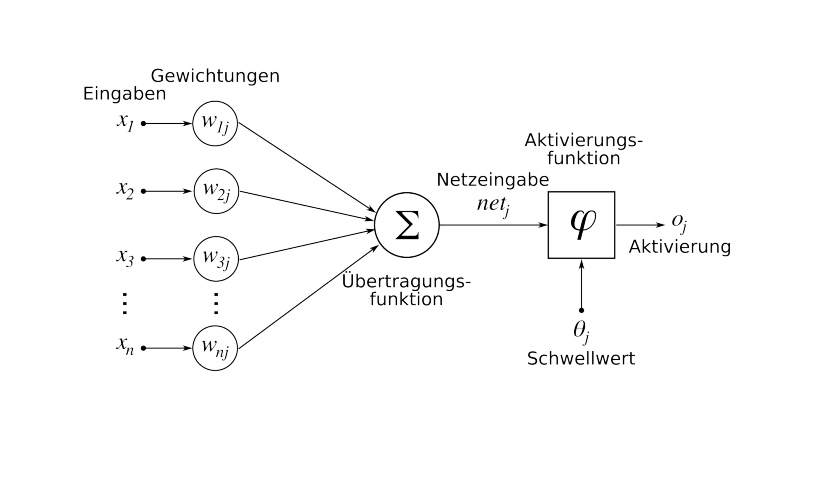
\includegraphics[width=\textwidth]{AufbauNN}
        \caption{Aufbau eines Neurons}
        \label{fig:AufbauNN}
    \end{figure}
    
    \noindent
    Die Eingangsfunktion berechnet aus verschiedenen Eingängen den effektiven Eingang, welcher dann weiter von der Aktivierungsfunktion verarbeitet wird.
    Diese effektive Eingabe ist dann die Netzeingabe in das Neuron.
    Meist wird die Netzaktivität \(net\) einfach als Summe aller Eingänge \(x\) und deren Gewichtungen \(w\) errechnet:
    \begin{equation}
        net = \sum_{i=0}^N x_i w_i
    \end{equation}
    \newline

    \noindent
    Die Aktivierungsfunktion dient zur eigentlichen Auswertung der Eingabe bzw. Netzaktivität.
    Diese erzeugt ein Aktivierungspotential, welches von der Ausgangsfunktion ausgewertet wird.
    \newline
    
    \noindent
    Die Ausgangsfunktion entscheidet schlussendlich ob das Neuron angeregt wird, oder nicht.
    Hierzu wird geprüft ob das Aktivierungspotential der Aktivierungsfunktion einen bestimmten Schwellenwert übersteigt.
    Dieser Schwellenwert wird mithilfe einer Schwellenwertfunktion errechnet. 
    Die Schwellenwertfunktion muss monoton wachsend sein, kann jedoch verschiedene Formen annehmen. 
    Sie kann linear verlaufen wie es beim Perzeptron der Fall ist, nicht-linear oder eine Sprungfunktion sein. 
    Durch eine nicht-lineare Funktion, wie die Sigmoid-Funktion lassen sich mächtigere neuronale Netze entwickeln, weshalb heuzutage meist eine solche zum Einsatz kommt.


    \subsubsection{Topologie}
    Bei einem neuronalen Netz sind dessen Neuronen über Synapsen, welche bestimmte Kantengewichte bzw. Biases haben, verbunden.
    Durch verschiedene Kantengewichte können Eingänge oder bestimmte Features priorisiert werden. 
    Dies bedeutet, dass Eingänge welche größeren Einfluss auf das erwartete Ergebnis haben, höher gewichtet werden können und somit stärker in das Ergebnis mit einbezogen werden.
    \newline

    \noindent
    Durch Verbindungen zwischen Neuronen ergeben sich verschiedene Topologien von Netzen:
    \begin{description}
        \item[Vorwärts-verkettete Netze (feed-forword)] bestehen aus verschiedenen Neuronen-Schichten (hidden layers), welche nur mit der nächst höheren Schicht verbunden sind. Somit verlaufen die Daten nur in eine Richtung, vom Eingang zum Ausgang.
        \item[Rekurrente Netze (\ac{RNN})] können aus mehreren Neuronen-Schichten bestehen, wobei hier Verbindungen in tiefere Schichten möglich sind. Dies bedeutet, dass Ergebnisse von vorherigen Durchläufen des Netzes als Eingang mit einbezogen werden können.
        \item[Voll-vernetzte Netze (fully connected)] sind neuronale Netze, bei denen alle Neuronen miteinander vernetzt sind. Wobei hierbei keine wirkliche Struktur erkennbar ist und ein sehr großer Rechenaufwand besteht.
    \end{description}

    \begin{figure}[H]
        \centering
        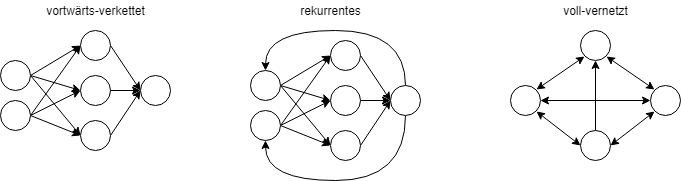
\includegraphics[width=\textwidth]{NetzTopologien}
        \caption{Netztopologien \cite{DrawIO}}
        \label{fig:NetzTopologien}
    \end{figure}


    \subsubsection{Lernen}
    Bei neuronalen Netzen ist das vorhandene Wissen durch die Kantengewichte repräsentiert.
    Daraus folgt, dass die verschiedenen Klassifikationen von neuronalen Netzen mit derselben Topologie, nur von den Kantengewichten abhängt.
    Dementsprechend lernt ein neuronales Netz durch sequentielles Anpassen der Gewichte.
    Dazu gibt es verschiedene Verfahren wie diese Gewichte angepasst werden können.
    \newline

    \noindent
    Beim \textbf{Backpropagation Lernen} werden in der Trainingsphase die Ergebnisse eines Durchlaufs mit den erwarteten Ergebnissen verglichen und der Ausgabefehler berechnet.
    Mithilfe dieses Fehlers wird nun schichtweise versucht den Fehler auf einzelne Neuronen bzw. Gewichte bis hin zur Eingabeschicht zurückzuführen.
    Danach werden nun bei verschiedenen Neuronen Änderungen der Gewichte durchgeführt, um den Fehler der Ausgabefehlerfunktion zu minimieren.
    Hierbei wird für jedes Gewicht mithilfe verschiedener Gradientenverfahren eine Änderung berechnet.
    \newline

    \noindent
    Beim \textbf{Batch Lernen} werden anders als beim Backpropagation Lernen nicht nach jedem Durchlauf des Netzes die Gewichte angepasst, sondern erst nachdem das Trainingsset komplett durchlaufen wurde.
    Dies kann zu weniger Genauigkeit führen, da nicht auf spezielle Eigenschaften einzelner Einträge eingegangen wird.
    Vorteil dieses Verfahren ist, dass sehr viel weniger Rechenaufwand benötigt wird und mehr Trainingsdaten in gleicher Zeit einbezogen werden können.
    
    \subsubsection{Perzeptron}
    Ein sehr einfaches neuronales Netz ist das Perzeptron, welches 1958 von Frank Rosenblatt entwickelt wurde.
    Das Perzeptron besteht aus zwei Eingabeparametern, welche in ein Neuron gegeben werden und von diesem mithilfe der Kantengewichte und der Aktivierungsfunktion eine Ausgabe liefert.

    Ein Beispiel ist die Abbildung des boolschen "`Und"'-Operators, welche wie in Abbildung \ref{fig:PerzeptronAND} mit einem Neuron dargestellt werden kann.
    Jedoch können mit einem Neuron nur sehr einfache Funktionen abgebildet werden. 
    Komplexere Funktionen können über mehrere Neuronen, beziehungsweise mehrere Schichten von Neuronen abgebildet werden.

    \begin{figure}[H]
        \centering
        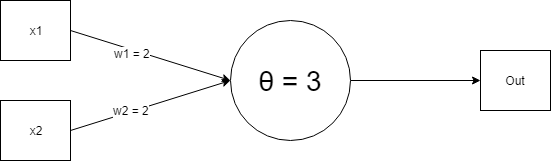
\includegraphics[width=\textwidth]{Perzeptron}
        \caption{UND-Operator als Perzeptron \cite{DrawIO}}
        \label{fig:PerzeptronAND}
    \end{figure}

    \begin{table}[H]
        \centering
        \begin{tabular}{|l|l|l|l|}
            \hline
            x1 & x2 & \( (x_1 * w_1) + (x_2 * w_2) \) & out \\
            \hline
            0 & 0 & \( (0 * 2) + (0 * 2) = 0 < 3 \) & 0 \\
            \hline
            0 & 1 & \( (0 * 2) + (1 * 2) = 2 < 3 \) & 0 \\
            \hline
            1 & 0 & \( (1 * 2) + (0 * 2) = 2 < 3 \) & 0 \\
            \hline
            1 & 1 & \( (1 * 2) + (1 * 2) = 4 < 3 \) & 1 \\
            \hline
        \end{tabular}
        \caption{Wahrheitstabelle des Perzeptron}
        \label{tabl:Perzeptron}
    \end{table}

    \paragraph{CNN - Convolutional Neural Network}
    \cite[Vgl. im Folgenden]{Robotics2}\\
    Eine weitere Form eines neuronalen Netzes ist ein \ac{CNN}.
    Diese Form findet häufig Anwendung in der Bilderkennung oder Bildklassifizierung.
    \newline

    Die Struktur eines \ac{CNN} besteht aus mehreren "`Convolutional Layern"' und einem "`Pooling Layer"'.
    Bei einem \ac{CNN} wird durch verschiedene Faltungsmatrizen eine mehrdimensionale Matrix ständig "`verkleinert"' (vgl. Abbildung \ref{fig:Typisch_CNN}).
    Dieser Prozess beschreibt eine Generalisierung der Eingabematrix, sodass als Ausgabe für jede Klassifizierungs-Klasse eine generalisierte, kleinere Matrix entsteht.
    
    Beim Lernen wird versucht diese Matrix so zu erzeugen, dass essentielle Eigenschaften für die jeweilige Klassifikation abgebildet werden.

    \begin{figure}[H]
        \centering
        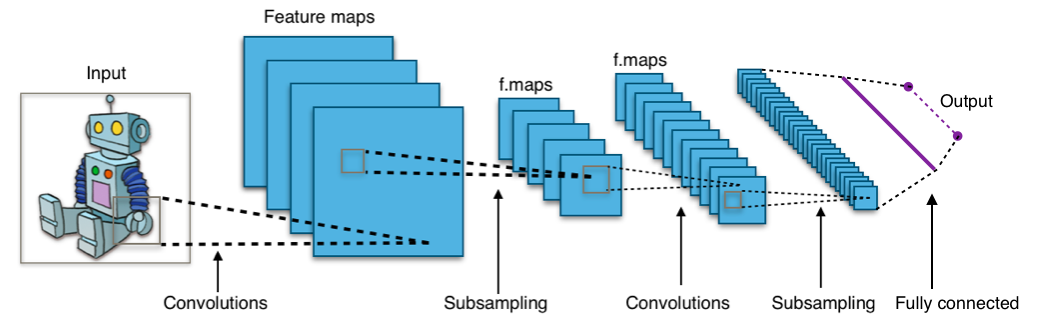
\includegraphics[width=\textwidth]{Typical_cnn}
        \caption[Typischer Aufbau eines CNN]{Typischer Aufbau eines \ac{CNN} \footnotemark }
        \label{fig:Typisch_CNN}
    \end{figure}
    \footnotetext{\url{https://upload.wikimedia.org/wikipedia/commons/6/63/Typical_cnn.png}}



\section{Physikalische Grundlagen} \label{physikalischeGrundlagen}
    Zur Messung der physikalischen Werte eines Stromnetzes wird ein WeSense-Messgerät\footnote{http://www.wesense-app.com/home-en/} verwendet.
    Dieses Messgerät misst sekündlich nach DIN EN50160\cite{WesenseManual} 9 verschiedene Parameter.
    Diese Parameter beinhalten die Spannung, die Frequenz sowie die ungeraden harmonischen Spannungsoberwellen bis zur 15ten\cite[S.2, Kapitel 1.2]{WesenseManual}.
    \newline

    Die DIN EN50160\cite{EN50160} gibt an wie sich die sieben ungeraden harmonischen Oberwellen aus der Spannung zusammensetzen.
    Harmonische Oberwellen sind reine sinusförmige Schwingungen, welche das n-fache einer Grundfrequenz sind.
    Addiert ergeben diese verschiedenen Oberwellen den gemessenen Wert (vgl. Abbildung \ref{fig:AddierteOberwwellen}).

    Die harmonischen Spannungsoberwellen werden als Oberschwingungspegel der Grundfrequenz in Prozent angegeben.
    Die Grundfrequenz \( f \), mit Geschwindigkeit \( V \) und Wellenlänge \( \lambda \), ergibt sich aus \( f = \frac{V}{\lambda} \).
    %Grundfrenquenz?

    \begin{figure}[H]
        \centering
        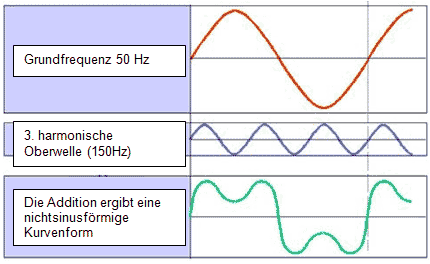
\includegraphics[width=0.6\textwidth]{herr_addition_grundwelle_3_harmonische_oberwelle}
        \caption[Addition von Oberwellen]{Beispiel für Addition von Oberwellen \footnotemark }
        \label{fig:AddierteOberwwellen}
    \end{figure}
    \footnotetext{\url{http://www.energie.ch/harmonische-oberschwingungen-netzqualitaet}}

    Netzteile, welche in verschiedenen Haushaltsgeräten eingebaut sind, verbrauchen je nach Nutzung mehr oder weniger Strom.
    Durch diesen Verbraucher sinkt oder steigt die Spannung im Netz.
    Auch beeinflusst jedes Netzteil die harmonischen Oberwellen auf eine andere Art und Weise.
    
    Durch diese zwei Einwirkungen auf das gesamte Stromnetz eines Haushalts sollte es folglich möglich sein Unterschiede zu erkennen.
    
    Jedoch könnten Komplikationen auftreten, da das Messgerät nur sekündlich Daten misst und möglicherweise Veränderungen der Parameter so minimal sind, das diese in der Zeitspanne nicht erkannt werden. 

    % \begin{figure}[H]
    %     \centering
    %     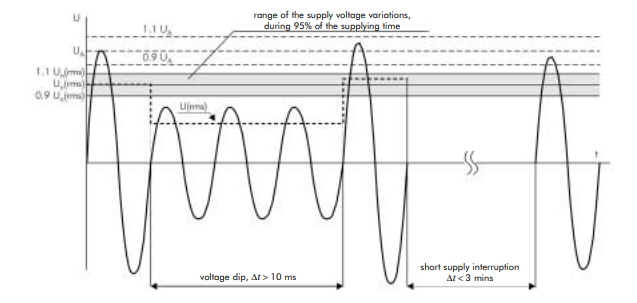
\includegraphics[width=\textwidth]{EN50160}
    %     \caption[EN5060 Harmonische Oberwellen]{Illustration of a voltage dip and a short supply interruption, classified according to%
    %     EN 50160; Un – nominal voltage of the supply system (rms), UA – amplitude of the supply%
    %     voltage, U(rms) – the actual rms value of the supply voltage \cite[S. 5]{EN50160}}
    %     \label{fig:EN50160_Hamonics}
    % \end{figure}

\section{Erhebung der Messdaten} \label{Messdaten}

    Um aussagekräftige Analysen und Klassifikationen über ein Stromnetz, beziehungsweise die Geräte in einem Stromnetz, mit maschinellem Lernen machen zu können, werden viele Trainings- und Testdaten benötigt.
    Die Daten bestehen aus verschiedenen physikalische Größen, die zu einem bestimmten Zeitpunkt in einem Stromnetz auftreten.
    Zu diesen Größen gehört die allgemeine Netzspannung, die Netzfrequenz und sieben harmonischen Oberwellen (vgl. \ref{physikalischeGrundlagen}).
    Um einen allgemeinen Überblick über den Verlauf der Netzaktivität zu erhalten, sowie verschiedene Zeiten und Geräte vergleichen zu können, müssen Daten über lange Zeiträume erhoben werden.\\
    \newline
    Das Messgerät, welches in Kapitel \ref{physikalischeGrundlagen} beschrieben wird, misst alle benötigten Werte und sendet diese über einen MQTT-Broker\footnote{Message Queuing Telemetry Transport} an einen Service, welcher die Daten aufbereitet und in einer MSSQL Datenbank abspeichert.
    Die Werte werden sekündlich gemessen und in die Datenbank gespeichert oder an registrierte Websocket-Verbindungen gesendet.
    \newline

    \begin{figure}[h]
        \centering
        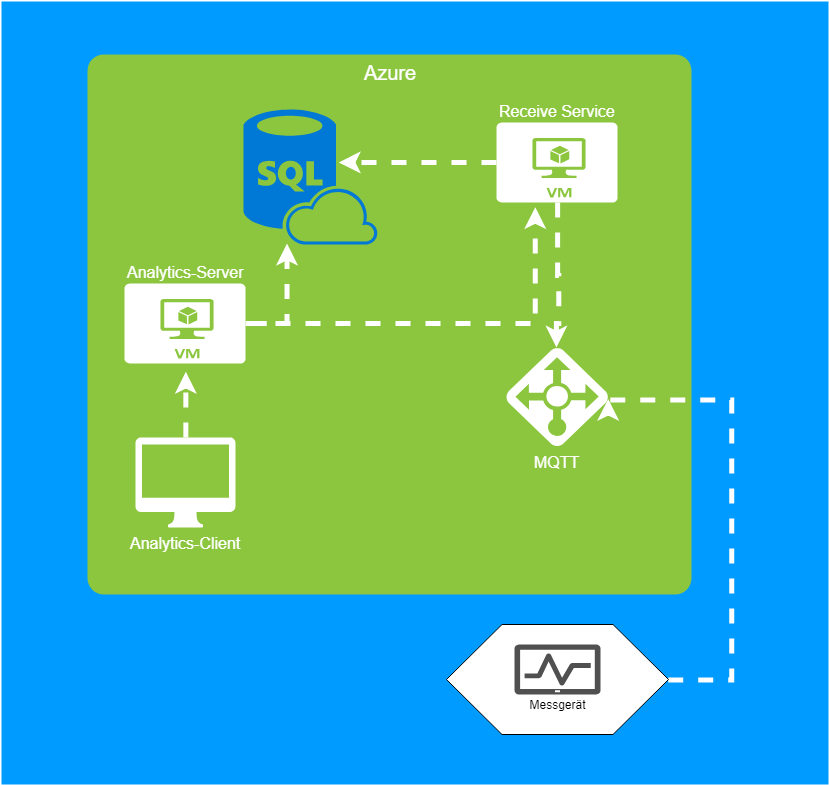
\includegraphics[width=0.7\textwidth]{WeSenseArchitecture}
        \caption{Architektur zur Abspeicherung der Daten \protect\cite{DrawIO}, \protect\cite{Tensorflow}}
        \label{fig:ArchitectureWesense}
    \end{figure}

    \subsection*{Klassifikation der Messdaten}\label{KlassifikationDerMessdaten}

        Wie in Abschnitt \ref{Messdaten} beschrieben, sind die rohen Messdaten in einer Datenbank abgespeichert.
        Zusätzlich werden nun zur Identifikation der Geräte, sowie zum maschinellen Lernen genau definierte Zeiträume benötigt, in denen bestimmte Geräte aktiv waren.
        Dies bedeutet, dass jedem Zeitpunkt ein oder mehrere Geräte zugewiesen werden. 
        Die einem Gerät zugewiesenen Daten werden im weiteren Verlauf gelabelte Daten genannt.\\
        \newline
        Die gelabelten Daten können manuell oder automatisiert erhoben werden.

        Die manuelle Erhebung der Daten erfordert eine Person, welche Zeiten zu denen sicher Geräte aktiv, waren manuell kennzeichnet.

        Um Daten automatisiert zu erheben wird ein weiteres Messgerät pro Haushaltsgerät benötigt.
        Dieses Messgerät müsste zwischen dem zu messenden Gerät und dem Stromnetz zwischengeschalten werden, um das Gerät zu klassifizieren sobald Strom fließt.
        Die automatisierte Methode ermöglichst es präzisere Klassifikationen, als auch mehr Zeitspannen und Haushaltsgeräte gleichzeitig zu erfassen, und ist somit die bevorzugte Methode.

        Jedoch müsste für die automatisierte Methode ein weiteres Gerät entwickelt werden, weshalb für diese Arbeit diese manuelle Methode gewählt wird.\\
        \newline

        Für die manuelle Datenerfassung wurde eine progressive Web-Applikation(vgl. Abbildung \ref{fig:WebApp1}, API: \cite{WesenseAPIRepo}, GUI: \cite{WesenseGUIRepo}) mit einer einfachen MySQL-Datenbank im Backend erstellt.
        Mithilfe dieser App können die Daten sehr einfach über ein mobiles Endgerät erfasst und abgespeichert werden.
        \newline

        \begin{figure}[h]
            \centering
            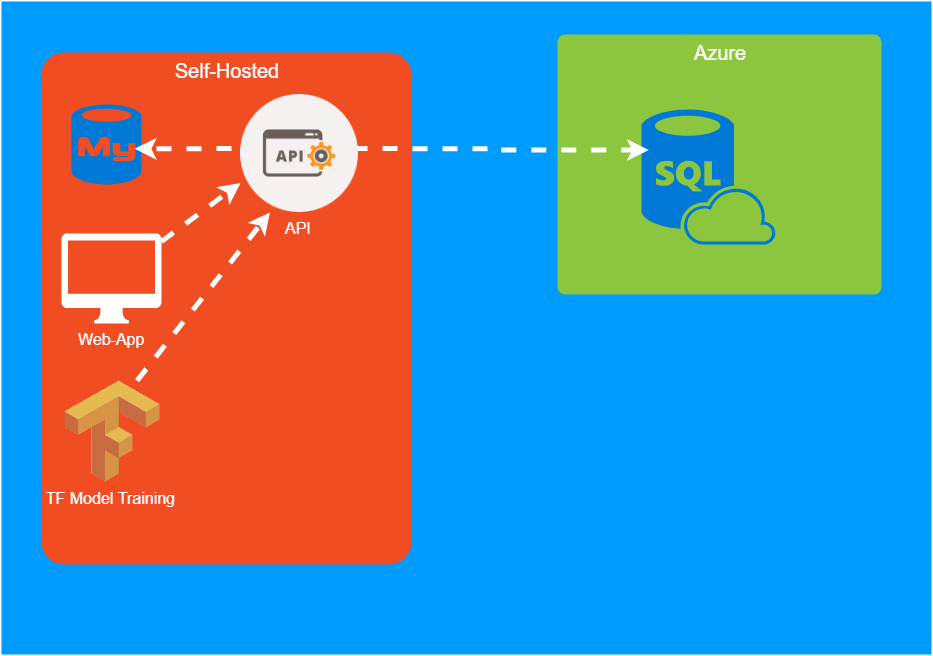
\includegraphics[width=1.0\textwidth]{ArchitectureTraining}
            \caption{Architektur zum Training der neuronalen Netze \protect\cite{DrawIO}, \protect\cite{Tensorflow}}
            \label{fig:ArchitectureTraining}
        \end{figure}

        Abbildung \ref{fig:ArchitectureTraining} zeigt die Einbindung der GUI und des API\-Servers in die Architektur der Messdatenspeicherung.
        Die entwickelte Applikation besteht aus einer GUI, welche eine Website ist, und eine Visualisierung für den API\-Server darstellt.
        Der API\-Server bildet das Verbindungsstück zwischen den klassifizierten Zeiträumen und den eigentlichen Daten des Messgerätes.
        Die Website, welche auf dem Polymer\-Framework\footnote{\url{https://www.polymer-project.org/}} basiert, ist somit nur eine Anzeige für die Funktionen des API-Servers.
        Sie bietet mehrere Seiten zur manuellen Klassifikation der Geräte, sowie verschiedene Visualisierungen(vgl. Anbschnitt \ref{VisualisierungWebApp}) zur Analyse der klassifizierten Zeiträume.

        \begin{figure}[h]
            \centering
            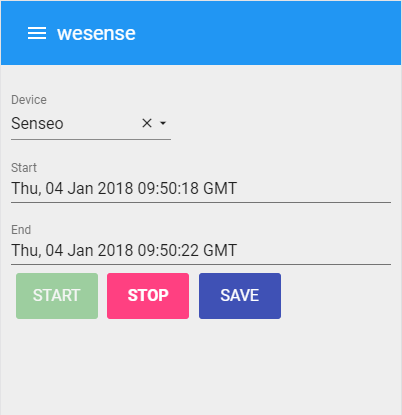
\includegraphics[width=0.5\textwidth]{WesenseConveyWebApp}
            \caption{Screenshot der progressive Web-App}
            \label{fig:WebApp1}
        \end{figure}

\section{Visualisierung}\label{VisualisierungWebApp}

        Zusätzlich zur manuellen Erhebung der Daten, sowie zur besseren Analyse der Daten, wurden verschiedene Visualisierungsmöglichkeiten implementiert.
        Einerseits können die verschiedenen physikalischen Größen eines Gerätes zu einem bestimmten Zeitpunkt miteinander verglichen werden.
        Andererseits können auch bestimmte Größen zu gelabelten Zeiträumen eines Gerätes verglichen und analysiert werden. 
        Durch diese Visualisierung können Gemeinsamkeiten bestmöglich in unterschiedlichen Größen oder Zeiten erkannt werden.\\
        \newline
        Es werden verschiedene Diagramme sowie Normalisierungen der Daten zur Analyse bereitgestellt.
        Die Analyse der Daten können in verschiedenen Diagrammen und Normalisierungen dargestellt werden:
        \begin{itemize}
            \item sekündlich in einem Liniendiagramm
            \item in Datenpunkten (Klassen), welche frei wählbar sind
            \item Histogramme mit verschiedenen Klassen
        \end{itemize}

        \begin{figure}[h]
            \centering
            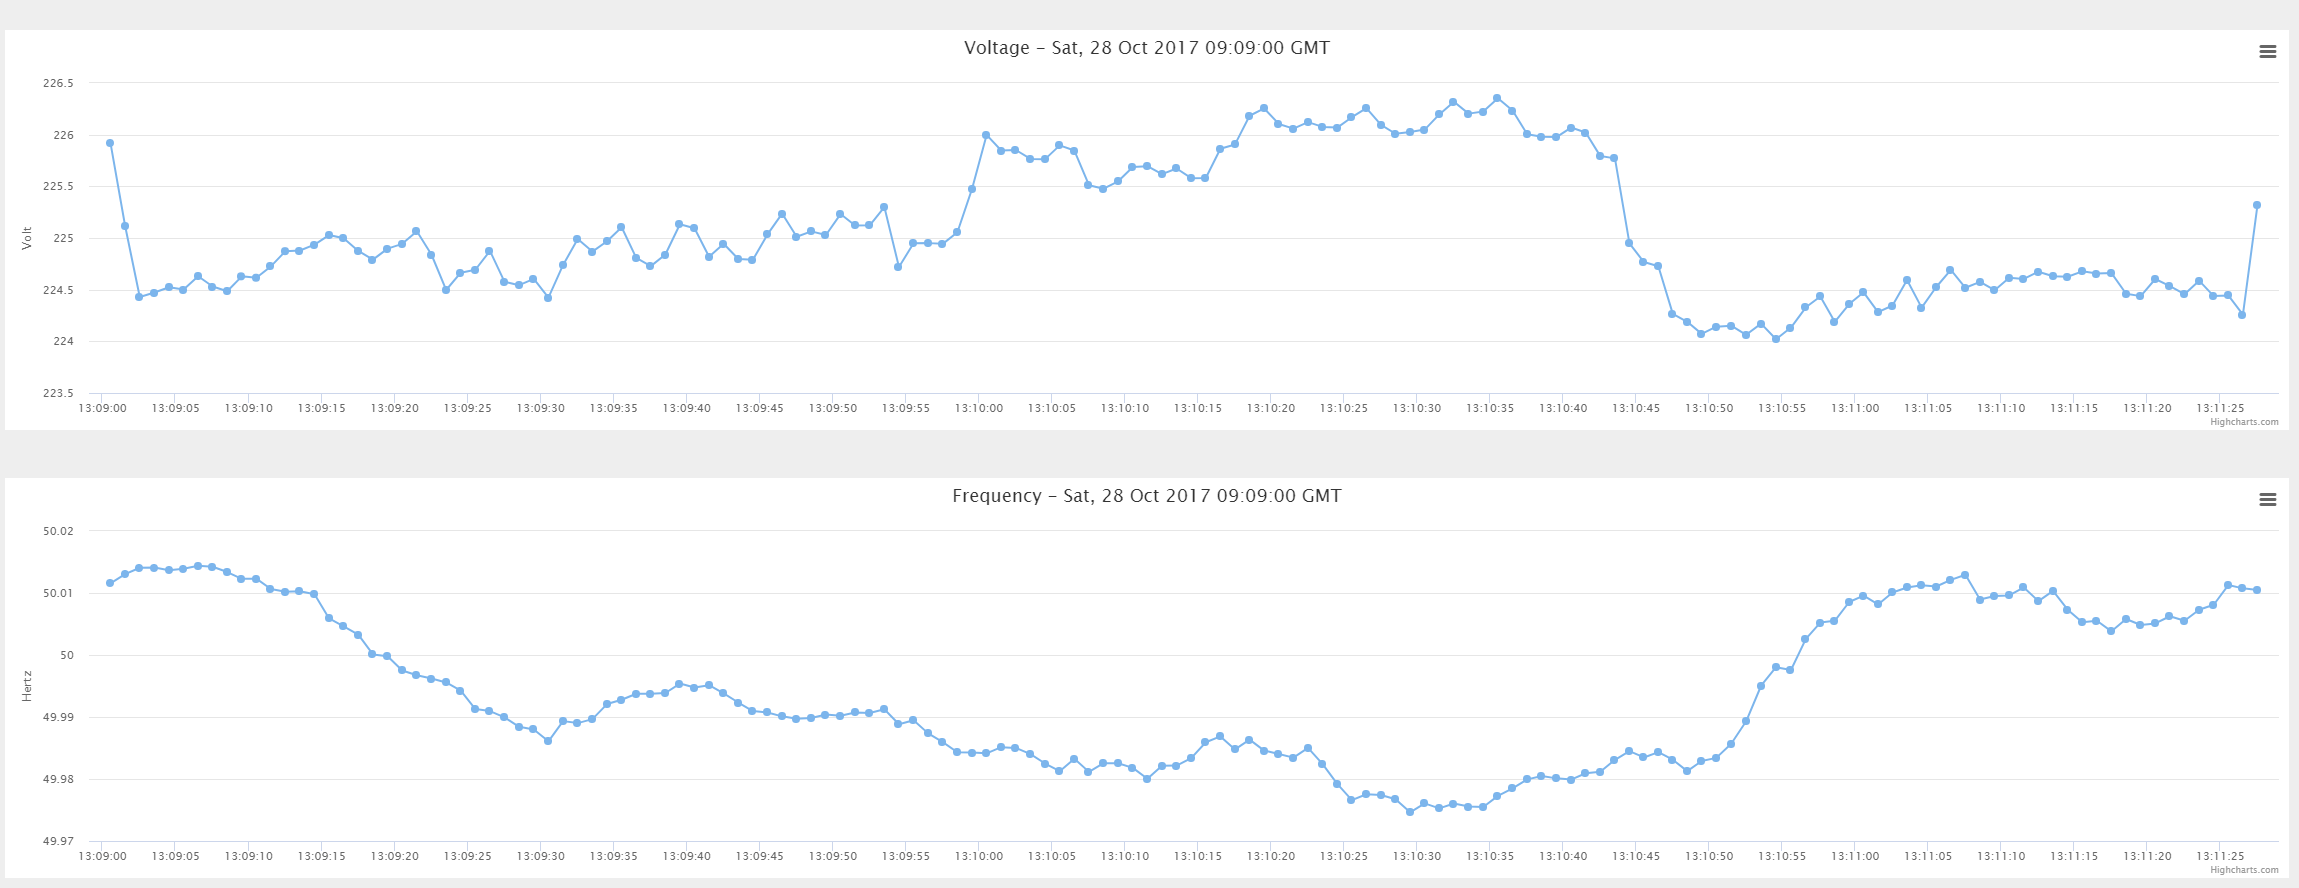
\includegraphics[width=0.75\textwidth]{WesenseConveylineChart}
            \caption{Screenshot eines gelabelten Zeitraumes aus der Web-App}
            \label{fig:WebApp2}
        \end{figure}
